\documentclass[a4paper,12pt]{article}
\parindent 0pt
\parskip 1mm
\usepackage{amsmath}
\usepackage[dvips]{epsfig}

\begin{document}

\begin{center}

{\Large\bf CN 510 - Principles and Methods of Cognitive and Neural Modeling}

\bigskip

{\large\bf Assignment \# 7}
\smallskip

{\large\bf John Joseph}
\end{center}

\bigskip
{\bf The Outstar Network}
\bigskip

This week we are modelling an Outstar Network with three border cells. We supply each border cell with a distinct inputs $I$ and will comment on how the pattern of inputs is stored across the system as a whole. 

\vspace{2mm}

The network is described by one source cell and several sink (or border cells); the relative strength of our input $I$ to border cell $i$ determines the synaptic weight between that border cell and the source cell. The source cell recieves an input, and behaves following the equation

\begin{equation}
  \frac{dx_o}{dt} = -A_0x_0+I_0
\end{equation}

The border cells behave as

\begin{equation}
  \frac{dx_i}{dt} = -Ax_i+B[x_0(t-\tau) - \Gamma]_+w_{0i} + I_i
\end{equation}

And their synaptic weights behave as

\begin{equation}
  \frac{dw_{0i}}{dt} = -Cw_{0i}+D[x_o(t-\tau)-\Gamma]_+x_i
\end{equation}

\bigskip
{\bf Analysis}
\bigskip

In order to analyze the long term behavior of our equations, let's define some terms. Our source sampling signal, which controls how and when our border cells recieve input from the source cell, can be written as follows:

\begin{equation}
  S_0(t) = [x_0(t-\tau)-\Gamma]_+
\end{equation}

The little plus sign means we are taking the maximum value between the value within the brackets and zero, or in other words ensuring the value is greater than or equal to zero. We can also solve our differential equation for the source cell using methods that have stood the test of time; doing so, we see that

\begin{equation}
  x_0(t) = \frac{I_0}{A_0}(1-e^{-A_ot})
\end{equation}

Once our sampling signal $S_0(t)$ becomes positive, we can solve for the equilibrium solutions of our border cell activations and synaptic weights by setting their rates of change equal to zero:

\begin{equation}
  -Ax_i+BS_0(t)w_{0i} + I_i = 0
\end{equation}
\begin{equation}
  -Cw_{0i}+DS_0(t)x_i = 0
\end{equation}

This is a system of two equations with two unknowns; solving for one variable in terms of the other and plugging back in, we find that

\begin{equation}
  x_i=\frac{CI_i}{CA-BDS_o(t)^2}
\end{equation}
\begin{equation}
  w_{0i}=\frac{DI_i}{A-BDS_o(t)}
\end{equation}

The first thing to note here is that the long term behavior of our sampling signal $S_0(t)$ will be 

\begin{equation}
  S_{0eq}(t) = \frac{I_0}{A_0} - \Gamma
\end{equation}

The second thing is that we are asked to determine, and will generally be concerned with, the behavior of the pattern variables representing weight and activation rather than these variables themselves. I have not solved for the pattern variables, but what I have solved for should be indicative of their overall behavior. 

\vspace{2mm}

The pattern variables of our system should tell what the activations and synaptic weights of our border cells should be relative to one another; noting that in both the weight and activaton expressions the only variable that really changes from border cell to border cell is the input $I_i$, we can conclude that the long term behavior of our pattern variables for both the activations and their weights should be proportional to, if not equal to, the pattern variable representing our input $I_i$. 

\vspace{2mm}

Therefore, the equilibrium values of our pattern variables for the weight and activation of our border cells should bear a strong resemblance to the pattern variables of our input pattern $I_i$. The is the principal result outlined in the Outstar Learning Theorem, and implies that our system has ``perfectly learned'' the input pattern which we provided. We will now run a computational simulation to see whether or not this is the case. 

\bigskip
{\bf Computational Work}
\bigskip

I honestly thought I'd be able to solve the border cell equations analytically and use the Rotter-Diessman integration method, but I wasn't able to find a solution. I'd still be curious to know what it was, but since I was unable to find itI integrated the equations using Runge-Kutta 4. Given that we were working with a system of equations, care was taken to ensure that the updates occured in a synchronized manner. 

\vspace{2mm}

The first tests were carried out with an A value of 5, and below you can see the normalized and unnormalized plots. Each border cell is plotted along with its input, plotted in the same color. You can see that, although both plots maintain relative position as a function of the input, the normalized plot actually approaches (and reaches) the exact input values we gave it. 

\vspace{2mm}

The same is true for the weight graph, which follows from our analysis of the long term behavior of the system. Both the weights and the activations preserve the input pattern, and in the case of the pattern variables the weight and activation approach the exact values of their input. 

\vspace{2mm}

When we change A to 0.5, some confusing things happened. If you take a look at our differential equtions, a sufficently low value will actualy cause the rate of change to be positive. This will cause our system to increase without bound, and the value of 0.5 is low enough to send our system into such a state. This is exactly what we see in our unnormalized plots, but when I normalized the plot I got some strange results. 

\vspace{2mm}

I wasn't sure whether or not an unstable outstar network would still uphold the Outstar Learning Theorem. It seems as though it did, to a degree, although only one of the neurons (i=3) seems to have converged to its expected value. The other two went either slightly above or slightly below the input value, although normalization was maintained (the sums were equal to 1). 

\begin{center}
\begin{figure}[h!]
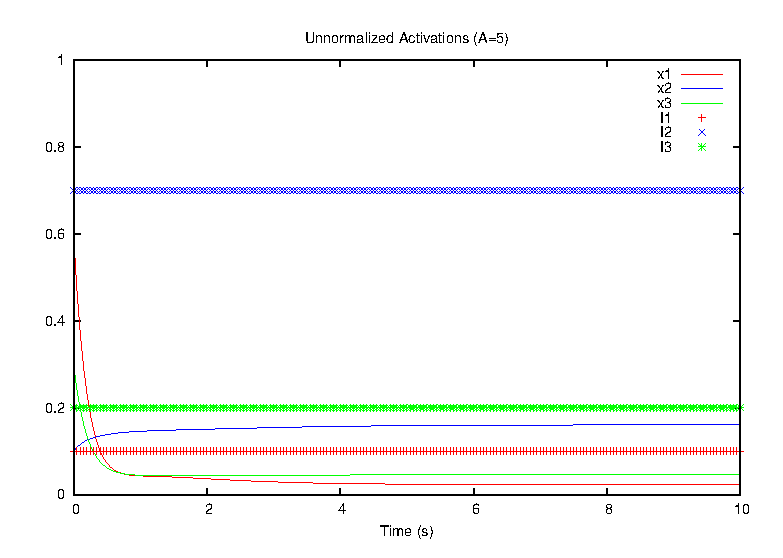
\epsfig{file=data/figures/ux1,width=16cm,height=11cm}
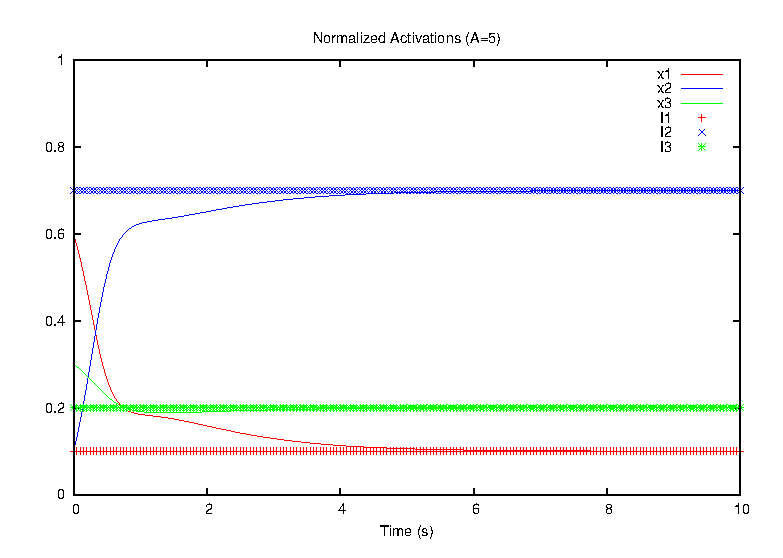
\epsfig{file=data/figures/nx1,width=16cm,height=11cm}
\end{figure}
\end{center}

\begin{center}
\begin{figure}[h!]
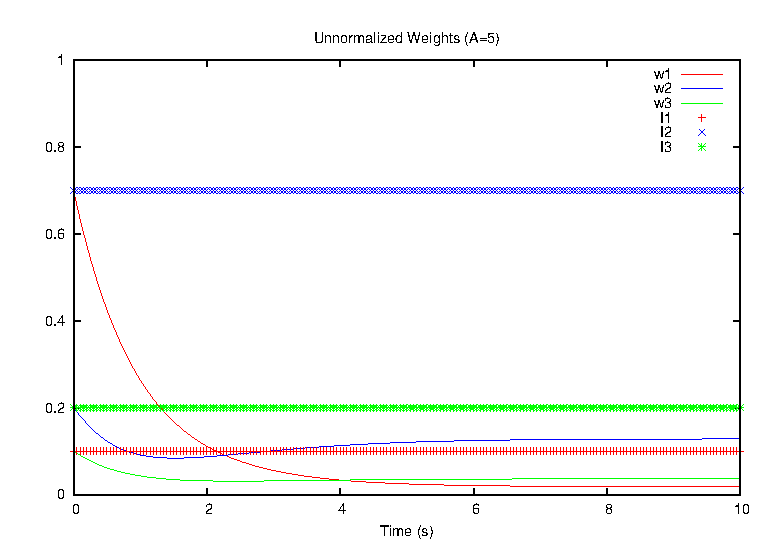
\epsfig{file=data/figures/uw1,width=16cm,height=11cm}
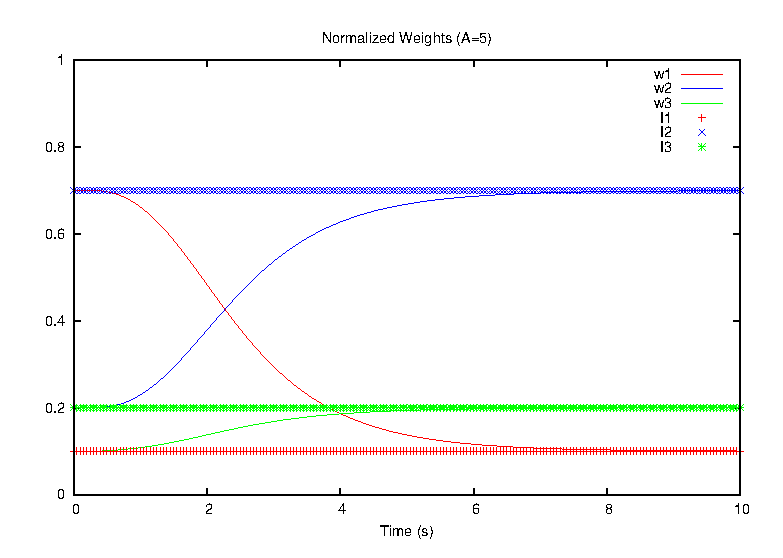
\epsfig{file=data/figures/nw1,width=16cm,height=11cm}
\end{figure}
\end{center}

\begin{center}
\begin{figure}[h!]
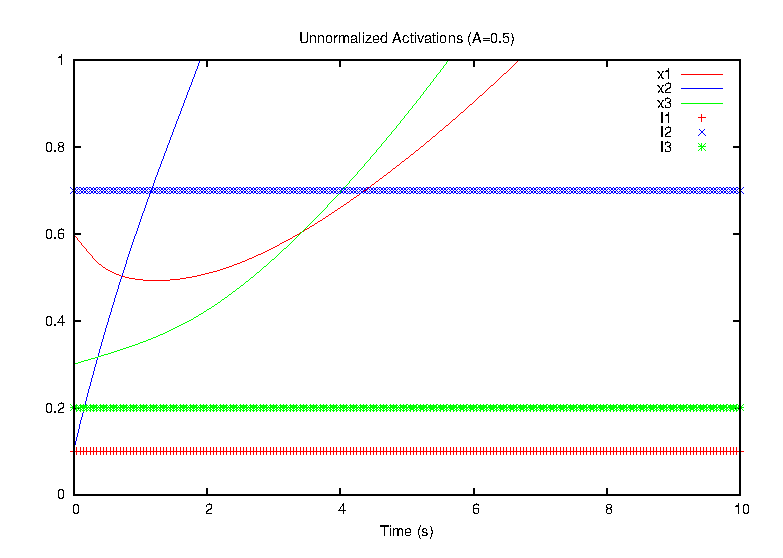
\epsfig{file=data/figures/ux2,width=16cm,height=11cm}
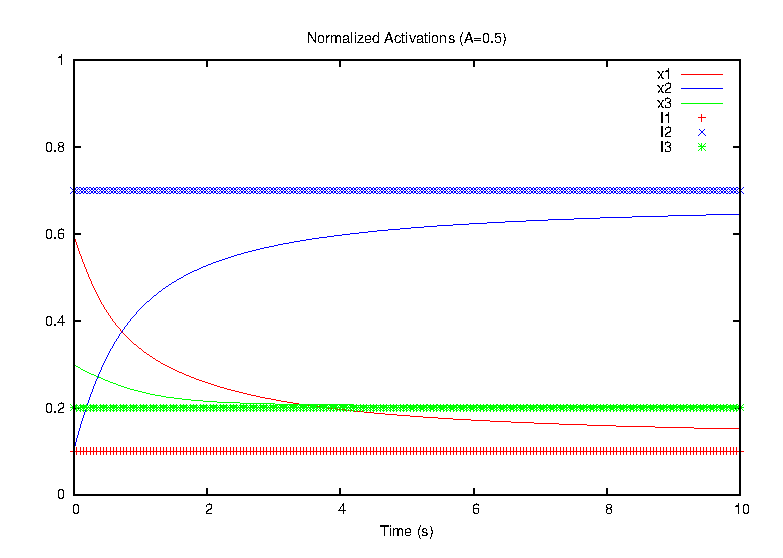
\epsfig{file=data/figures/nx2,width=16cm,height=11cm}
\end{figure}
\end{center}

\begin{center}
\begin{figure}[h!]
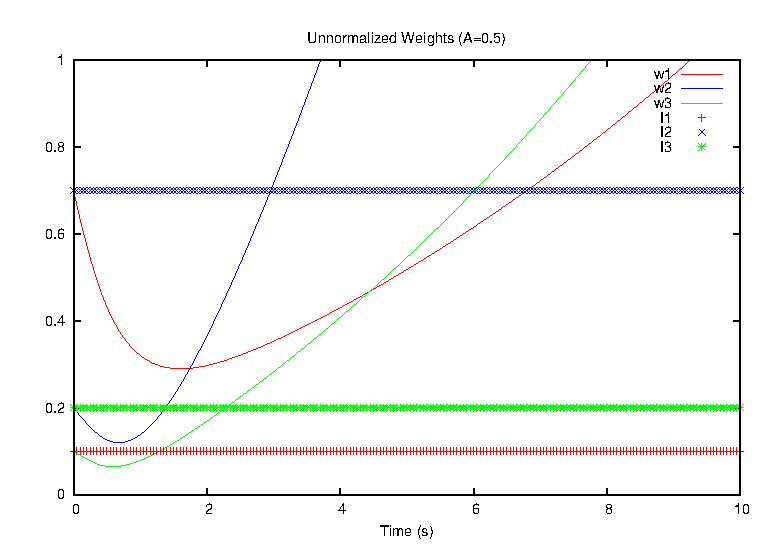
\epsfig{file=data/figures/uw2,width=16cm,height=11cm}
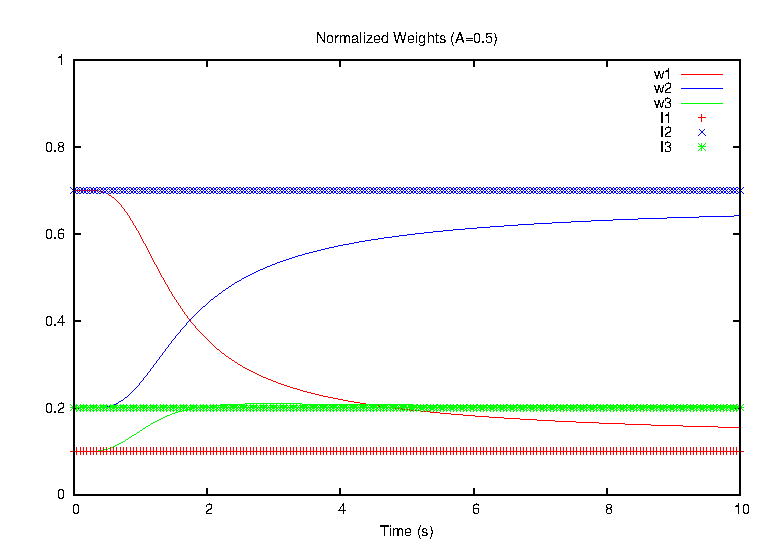
\epsfig{file=data/figures/nw2,width=16cm,height=11cm}
\end{figure}
\end{center}

\vfil\eject

{\bf Summary}
\bigskip
The strange behavior of my last two normalized plots still bugs me, and I cannot account for the slight changes in only two of the neurons. Perhaps I missed something in class, but I think it's due to some bug in my code. I haven't found it, and I didn't change anything but A between runs. Still, the results are there; out of curiosity I ran the simulation to $t=10000$, but the values did not get any closer. 

\vspace{2mm}

Despite that hiccup, the Outstar Learning Theorem was preserved, and my rudimentary analysis seemed to hold up. When we did not normalize the plot, we got results that were similar in form but not value to the input pattern; looking at my equilibrium solutions, we can see that our input values are divided by something greather than 1, so this makes sense. 

\vspace{2mm}

When we normalize the plot we see that our activations and weights go straight to the inputs, showing that the system has ``learned'' what we taught it. 

\end{document}
